\begin{figure*}[!t]
\begin{tabular}{c c c}
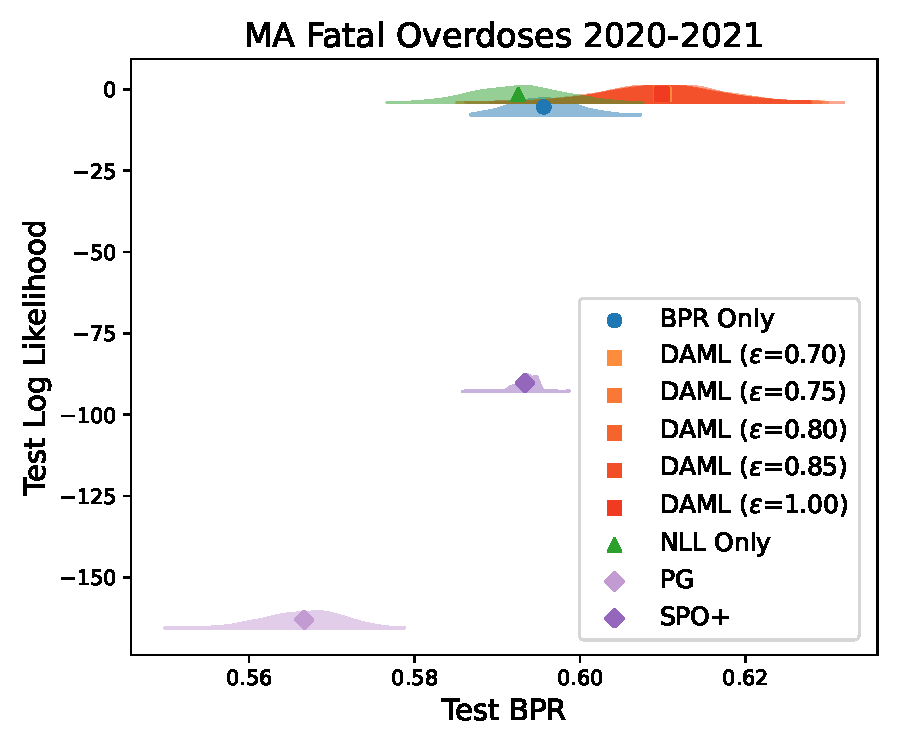
\includegraphics[width=.3\textwidth]{figures/MA_Frontier_PyEPO.pdf}
&
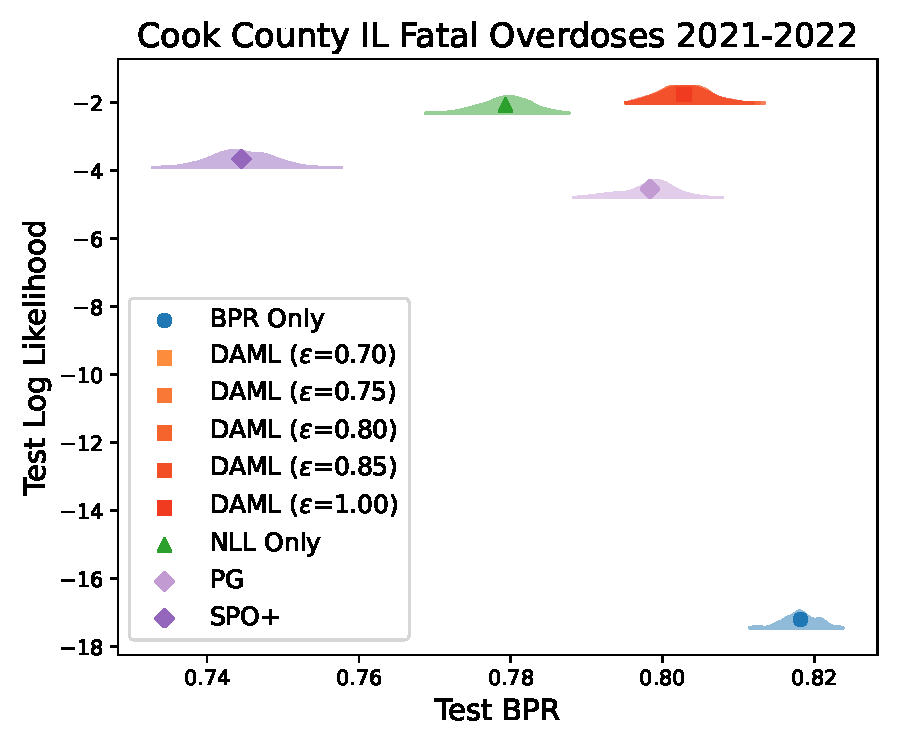
\includegraphics[width=.3\textwidth]{figures/Cook_Frontier_PyEPO.pdf}
&
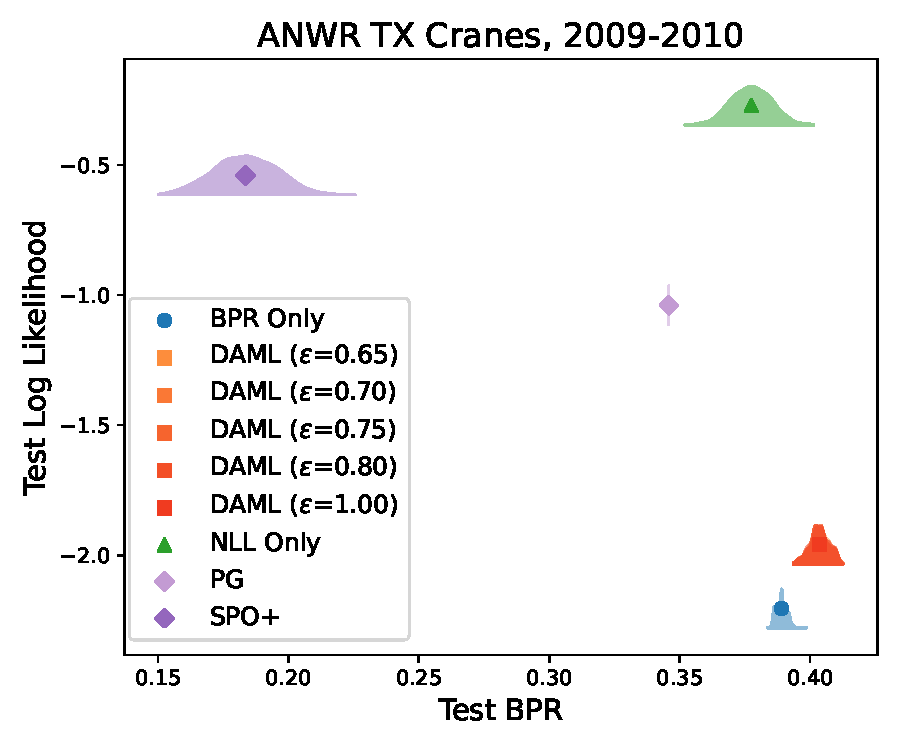
\includegraphics[width=.3\textwidth]{figures/AsurvFrontier.pdf}
\end{tabular}
\captionof{figure}[Pareto frontier of best possible reach (BPR) and log likelihood for real-world tasks.]{
    \textbf{Pareto frontier of best possible reach (BPR, x-axis) and log likelihood (LL, y-axis) for real-world tasks}. Higher is better on both axes. Each panel how the final models estimated by different training methods score on the test set of a forecasting task defined in Sec.~\ref{sec:results}. 
    To capture the stochasticity of BPR due to our sampling-based ranking estimator, for each model we show an estimated density for BPR over 1000 trials. Uncertainty in this plot only corresponds to uncertainty in BPR, log likelihood is a point estimate.
    In all three tasks, our proposed decision-aware ML (DAML) delivers better top-K decisions as measured by BPR than ML estimation. DAML also delivers likelihood comparable to ML methods and \emph{much better} than directly optimizing BPR. In the Cranes dataset, the DAML objective surprisingly offers better BPR than the BPR-only objective, although the magnitude of this difference is small and perhaps due to the small-scale and sparsity of this dataset.  \\
    }
%end caption
\label{fig:Frontier}
\end{figure*}

%Tasks are (from left to right), \emph{MA Fatal Overdoses} (left), \emph{Cook County IL Fatal Overdoses} (center), and \emph{ANWR TX Cranes} (right).
%    (Left) Results on the task of predicting the top 100 census tracts for fatal opioid-related overdoses for Massachusetts averaged over the years 2020-2021. (Middle) Results predicting the top 100 census tracts for fatal opioid-related overdoses for Cook County, averaged over the years 2021-2022. (Right) Results on the task of predicting the top 50 500m$^2$ grid squares averaged over \todo{TKTK} 2-month periods in \todo{TKTK}. 
%In all 3 cases, we see that the hybrid objective offers comparable or better performance as measured by BPR compared to models trained with maximum likelihood estimation, at much higher likelihoods compared to models trained to directly minimize BPR.
